\documentclass{article}
\usepackage{amsmath}
\usepackage{array}
\usepackage{color}
\usepackage{graphicx}
\usepackage{float} %utiliser H pour forcer a mettre l'image ou on veut
\usepackage{lscape} %utilisation du mode paysage
\usepackage{mathbbol} % permet d'avoir le vrai symbol pour les reels grace a mathbb
\usepackage{enumerate}
\usepackage{marvosym}
\usepackage{moreverb} % permet d'utiliser verbatimtab : conservation la tabulation
\usepackage{url}


\setlength {\textwidth}{16cm}
\setlength {\textheight}{21cm}
\setlength {\oddsidemargin}{0cm}
\setlength{\headsep}{5pt} 

\newcommand\bn{\boldsymbol{\nabla}}
\newcommand\bo{\boldsymbol{\Omega}}
\newcommand\br{\mathbf{r}}
\newcommand\la{\left\langle}
\newcommand\ra{\right\rangle}
\newcommand\bs{\boldsymbol}
\newcommand\red{\textcolor{red}}

\renewcommand{\(}{\left(}
\renewcommand{\)}{\right)}
\renewcommand{\[}{\left[}
\renewcommand{\]}{\right]}


\begin{document}
\title{}
\author{Bruno Turcksin} 
\date{}
\maketitle

\tableofcontents

% Cross sections chapter
\section{Cross sections}
\red{ATTENTION PAS CONSISTENT DANS L'UTILISATION DES TAU. CERTAINS DEVRAIENT
ETRE E... EN FAIT TOUS SAUF LE PREMIER.}\\
\red{CHECK ALL THE $\Sigma_{t,s}$}\\
\red{rajouter les references des formules des sections efficaces}\\
\red{probablement des s en trop dans certaines formules}
\subsection{Physics of the interactions}

\begin{description}
\item [Thomson scattering :] an electron, assumed to be free, oscillates
classically in response to the electric vector of a passing electromagnetic
wave. The oscillating electron promptly emits photons of the same frequency as
the incident wave. The net effect of Thomson scattering is the redirection of
some incident photons with no transfer of energy to the medium. Thomson
scattering represents the low-energy limit of Compton scattering, as the
incident photon energy approaches zero \cite{radiation}.
\item [Raleigh scattering :] the scattering results from the combined,
coherent action of an atom as a whole. The scattering angle is usually very
small. There is no appreciable loss of energy by the photon to the atom,
which, however, does ``recoil" enough to conserve momentum \cite{radiation}.
\item [photo-electric effect :] a photon undergoes an interaction with an
absorber atom in which the photon disappears. An energetic photoelectron is
ejected from one of the bound shells of the atom. For gamma rays of
sufficient energy, the most probable origin of the photoelectron is the $K$
shell of the atom. The photoelectron appears with an energy given by :
\begin{equation}
E_{e^-} = h\nu -E_b
\end{equation}
where $E_b$ represents the binding energy of the photoelectron in its original
shell. The interaction leaves an ionized absorber atom with a vacancy in one
of its bound shells. This hole is quickly filled through the rearrangement of
electrons from other shells of the atom. Therefore, one or more X-ray photons
may also be generated. In some fraction of the cases, the emission of Auger
electrons may substitute for the X-ray. 
\begin{figure}[H]
\centering
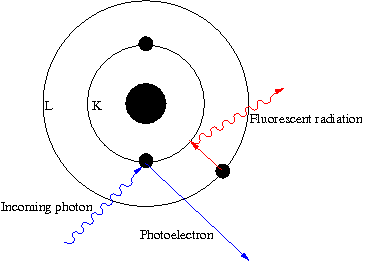
\includegraphics[width=0.5\linewidth]{./Cross_Sections/images/photoelectric}
\caption{Photoelectric effect}
\end{figure}
The photoelectric process is the
predominant mode of interaction for photons of relatively low energy. The
process is more important for high atomic number $Z$.The probability of
photoelectric absorption $\tau$ depends on $Z$ and $h\nu$ as :
\begin{equation}
\tau \propto \frac{Z^n}{\(h\nu\)^3}
\end{equation}
where $n$ varies between 4 and 5. The photoelectric interaction is most likely
to occur if the energy of the incident photon is just greater than the binding
energy of the electron with which it interacts.
\item [fluorescence :] fluorescence is a process in which some of the energy
of a photon is used to create a second photon of less energy.
\item [Compton effect :]  a Compton interaction is one in which only a portion
of the energy is absorbed and a photon is produced with reduced energy. This
photon leaves the site of the interaction in a different direction from that
of the original photon. If a photon of energy $h\nu$ and momentum
$\frac{h\nu}{c}$ is a incident on a stationary, free electron, after the
collision, the photon is scattered at an angle $\theta$ with energy $h\nu'$.
\begin{figure}[H]
\centering
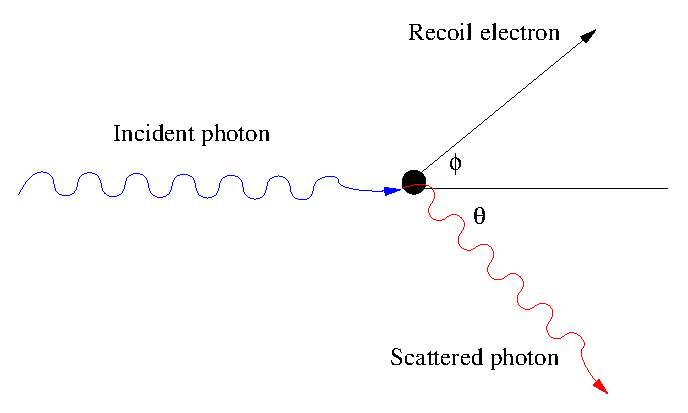
\includegraphics[width=0.5\linewidth]{./Cross_Sections/images/compton}
\caption{Compton effect}
\end{figure}
The Compton shift is given by :
\begin{equation}
\Delta \lambda = \lambda'-\lambda = \frac{h}{mc} \(1-\cos \theta\)
\end{equation}
The Klein-Nishina formal gives the differential cross section of photons
scattered from a single free electron :
\begin{equation}
\frac{d \sigma}{d\bo} = \frac{k_0^2 e^4}{2 m_e^2
c^4}\(\frac{\nu'}{\nu}\)^2\(\frac{\nu}{\nu'}+\frac{\nu'}{\nu}-\sin^e \theta\)
m^e sr^{-1}
\end{equation}
where $\frac{d\Sigma}{d\bo}$ is the differential scattering cross sections,
$k_0 = \frac{1}{4\pi \epsilon_0}$, $\epsilon_0$ is the vacuum permittivity,
$e$ is the elementary charge, $m_e$ is the mass of an electron and $c$ is the
speed of light in vacuum \cite{radiation}.
\item [Auger electron :] an atom in which an L electron makes a transition to
fill a vacancy in the K shell does not always emit a photon. An other L
electron can be ejected from the atom, thereby leaving two vacancies on the L
shell. The electron eject by the atom is called an Auger electron.
Auger-electron emission is favored over photon emission for elements of low
atomic number. The original inner-shell vacancy in an Auger-electron emitter
can be created by orbital electron capture, internal conversion, or
photoelectric effect. Auger cascades can occur in relatively heavy atoms, as
inner-shell vacancies are successively filled by the Auger process, with
simultaneous ejections of the more loosely bound atomic electrons.
\item [Bremsstrahlung :] is an electromagnetic radiation produced by a sudden
slowing down or deflection of charged particle (especially electrons) passing
through matter in the vicinity of the strong electric fields of atomic nuclei.
The efficiency of bremsstrahlung in elements of different atomic number $Z$
varies nearly as $Z^2$.
\item [Collisional stopping power :] the collisional stopping power for
electrons and positrons can be \hbox{written :}
\begin{equation}
\(-\frac{dE}{dx}\)_{col}^{\pm} = \frac{4\pi k_0^2 e^4 n}{m_e c^2 \beta^2}
\[\ln \(\frac{m_e c^2 \tau \sqrt{\tau+2}}{\sqrt{2}I}\)+F^{\pm}\(\beta\)\]
\end{equation}
where :
\begin{equation}
F^-(\beta) = \frac{1-\beta^2}{2} \[1+\frac{\tau^2}{8} - (2\tau +1 )\ln 2\]
\end{equation}
is used for electrons and :
\begin{equation}
F^+\(\beta\) = \ln 2 - \frac{\beta^2}{24} \[23 + \frac{14}{\tau +2} +
\frac{10}{\(\tau + 2\)^2} + \frac{4}{\(\tau + 2\)^2}\]
\end{equation}       
for positrons. Here $n$ is number of electrons per unit volume in the medium,
$\beta = \frac{v}{c}$ is the speed of the particle relative to $c$, $I$ is the
mean excitation energy of the medium and $\tau = \frac{T}{m_e c^2}$ is the
kinetic energy $T$ of the particle expressed in multiples of the electron rest
energy $mc^2$.
\item[radiative stopping power :] At high beta-particle energies, the
radiation is emitted mostly in the forward direction, that is, in the direction
of travel if the beta particle. Unlike collisional energy losses, no single
analytic formula exists for calculating the radiative stopping power. At high
energies bremsstrahlung becomes the predominant mechanism of energy loss for
beta particles. The following approximate formula gives the ratio of radiative
and collisional stopping powers for an electron of total energy $E$, expressed
in MeV, in an element of atomic number \hbox{$Z$ :}
\begin{equation}
\frac{\(\frac{dE}{dx}\)_{rad}^-}{\(\frac{dE}{dx}\)_{col}^-} \approx
\frac{ZE}{800}
\end{equation}
At very high energies the dominance of radiative over collisional energy
losses gives rise to electron-photon cascade showers. Since bremsstrahlung
photon spectrum is approximately flat out to its maximum (equal to the
electron's kinetic energy), high-energy beta particles emit high-energy
photons. These, in turn, produce Compton electrons and electron-positron
pairs, which then produce additional bremsstrahlung photons, and so on. These
repeated interactions result in an electron-photon cascade shower, which can
be initiated by either a high-energy beta particle or a photon.
\end{description}

\subsection{CEPXS}
The principal interactions that electrons and photons can have, are
\cite{cepxs} :
\begin{description}
\item [electron-to-electron :] collisional scattering, knock-on production,
radiative scattering, elastic scattering and Auger production following impact
ionization.
\item [electron-to-photon :] bremsstrahlung production and fluorescence
production following impact ionization.
\item [photon-to-photon :] incoherent scattering, coherent scattering (Thomson 
scattering and Raleigh scattering) and fluorescence production following
photoionization.
\item [photon-to-electron :] photoelectric production, Compton electron
production, pair production and Auger production following photoionization.
\item [photon-to-positron :] pair production.
\item [positron-positron :] collisional scattering, radiative scattering and
elastic scattering.
\item [positron-to-photon :] bremsstrahlung production, fluorescence
production following impact ionization and annihilation radiation.
\item [positron-to-electron :] knock-on production and Auger production
following impact ionization.
\end{description}
CEPXS is a multigroup Coupled Electron-Photon cross-section (XS) generating
code. CEPXS was created to \cite{cepxs} :
\begin{itemize}
\item generate coupled electron-photon cross sections which can be used by
standard discrete ordinates code to solve electron-photon transport
calculations
\item model the same physical interactions as Version 2.1 of the
Integrated-TIGER-Series (ITS) code package.
\end{itemize}
Now we define \cite{barjon} :
\begin{itemize}
\item $\sigma$ is the microscopic cross section. It is the mean probability than a
particle interacts whit a nucleus per $cm^2$. The unit of $\sigma$ is the barn
which is $10^{-24}cm^2$.
\item $\Sigma$ is the macroscopic cross section. $\Sigma = N \sigma$ where $N$
is the number of atoms per $cm^3$. The unit of $\Sigma$ is $cm^{-1}$.
\end{itemize}
In CEPXS, most cross sections for compounds are constructed using \cite{cepxs} :
\begin{equation}
\Sigma_{comp} = \sum_i w_i \Sigma_i
\end{equation}
where $w_i$ is the weight fraction of the $i^{th}$ element in the compound.
However, the collisional stopping power of a compound cannot be expressed a
combination of elemental stopping powers.\\
The multigroup method involves a discretization of the particle energy domain
into energy groups :
\begin{figure}[H]
\centering
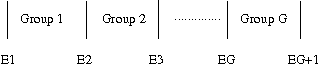
\includegraphics[width=0.5\linewidth]{./Cross_Sections/images/multigroup}
\caption{Multigroup}
\end{figure}        
where E1 $>$ E2 $>$ E3 $>$ $\cdots$ $>$ EG $>$ EG+1. EG+1 is the cutoff
energy. In CEPXS, different groups structures can be selected for photons and
electrons but the upper boundary energy and the cutoff energy are the same.\\
The multigroup angular flux, $\Psi^g\(\br,\bo\)$, is defined as :
\begin{equation}
\Psi^g\(\br,\bo\) = \int_{E^{g+1}}^{E^g} dE \Psi\(\br,\bo,E\)
\end{equation}
where $\Psi(\br,\bo,E)$ is the angular flux. The differential cross section,
$\Sigma_s(\br,E\rightarrow E',\mu)$ can be represented as :
\begin{equation}
\Sigma_s(\br,E\rightarrow E',\mu) = \sum_{l}^{\infty} \frac{2l+1}{4\pi}
\Sigma_{s,l}(\br,E\rightarrow E') P_l(\mu)
\end{equation}
where :
\begin{equation}
\begin{split}
\Sigma_{s,l}(r,E\rightarrow E') &= \int_{4 \pi} d\bo \Sigma_s\(\br,E\rightarrow
E',\mu\) P_l(\mu)\\
&= 2\pi \int_{-1}^1 d\mu \Sigma_s(\br,E\rightarrow,\mu) P_l\(\mu\)
\end{split}
\end{equation}
and $P_l$ are the Legendre polynomials. The multigroup-Legendre expansion
coefficients for the cross sections that describe scattering and production
interactions are stored by CEPXS in transfer matrices. For a differential
cross section, the expansion coefficients that are stored in the transfer
matrix of $L^{th}$-order are :
\begin{equation}
\Sigma_{s,L}^{g\rightarrow g'}\(\br\) = \frac{\int_{E^{g+1}}^{E^g} dE w(E)
\int_{E^{g'+1}}^{E^{g'}}} dE' \Sigma_{s,L}(\br,E\rightarrow
E'){\int_{E^{g+1}}^{E^g} dE w(E)}
\end{equation}
where $w(E)$ is the multigroup weighting function. $g$ is the row index of the
transfer matrix and $g'$ is the column index. In CEPXS the weighting function
is piece-wise constant in energy :
\begin{equation}
w(E) = c^g \textrm{ for } E^{g}\geq E \geq E^{g+1}
\end{equation}
where $c^g$ is a group-dependent constant. Therefore, the multigroup-Legendre
expansion coefficients become :
\begin{equation}
\Sigma_{s,L}^{g \rightarrow g'}\(\br\) = \frac{\int_{E^{g+1}}^{E^g}dE
\int_{E^{g'+1}}^{E^{g'}}dE' \Sigma_{s,L}\(\br,E \rightarrow E'\)}{\Delta E^g}
\end{equation}
where $\Delta E^g = E^g - E^{g+1}$.

The five types of reaction cross sections assembled by CEPXS are : total
$\(\Sigma_t\)$, absorption $\(\Sigma_a\)$, secondary production
$\(\Sigma_S\)$, energy deposition $\(\Sigma_E\)$ and charge deposition
$\(\Sigma_C\)$. For a reaction type $X$, the multigroup reaction rate is :
\begin{equation}
R_X^g = \int d\br \Sigma_X^g \Phi^g\(\br\)
\end{equation}
The reaction rate over all groups is :
\begin{equation}
R_X = \int_{g=1}^G R_X^g
\end{equation}
Energy-deposition cross sections are associated with every type of
interaction. These cross sections are defined as the net energy deposited in
the medium due to the interactions of particles in a group per unit
pathlength. These cross sections have units of energy per distance. The
energy-deposition multigroup cross sections for a scattering interaction could
be computed by :
\begin{equation}
\Sigma_{E,s}^g(\br) = \frac{\int_{E^{g+1}}^{E^g} dE' E
\Sigma_{s,0}(\br,E\rightarrow E') - \int_{E^{k+1}}^{E^k} dE \int_{E^{k+1}}^E
dE' E' \Sigma_{s,0}(\br,E\rightarrow E')}{\Delta E^g}
\end{equation}
However, it is not what is done in CEPXS where an effective energy-deposition
multigroup cross sections is defined :
\begin{equation}
\Sigma_{E,s}^g\(\br\) = \Sigma_{t,s}^g \(\br,E^{g,m}\) - \sum_{g'=1}^G
\Sigma_{s,0}^{g\rightarrow g'}\(E^{g',m}\)
\end{equation}
where $E^{g,m}$ is the midpoint energy of group $g$ and $\Sigma_{t,s}^g$ are
the total scattering multigroup cross \hbox{sections :}
\begin{equation}
\Sigma_{t,s}^g = \frac{\int_{E^{g+1}}^{E^g} dE \int_{E^{min}}^E dE'
\Sigma_{s,0} \(\br,E \rightarrow E'\)}{\Delta E^g}
\end{equation}
with the assumption that :
\begin{equation}
\Sigma_{s,0}(\br,E\rightarrow E') = 0 \textrm{     for }E' < E_{min}
\end{equation}
We can notice that :
\begin{equation}
\Sigma_{t,s}^g\(\br\) = \sum_{g'=1}^G \Sigma_{s,0}^{g \rightarrow g'}(\br)
\end{equation}
only when $E^{min} > E^{g+1}$

\subsubsection{Catastrophic collisional scattering}       
In CEPXS, inelastic scattering due to catastrophic collisions are modelled by
the M\o ller microscopic cross section, $\sigma^{CC}$. One of the assumptions
used in the derivation of the M\o ller cross section is that the incident
electron collides with a free atomic electron. The adequacy of this assumption
depends on how the energy of the incident electron compares to the binding
energy of the atomic electron with which it collides. For example, if the
incident-electron energy is on the order if the binding energy of an electron,
the assumption of zero binding is wrong. After an inelastic collision, two
electrons emerge. By convention, the particle with the higher energy is
considered to be the primary electron. The electron is the knock-on electron.
The M\o ller cross section can be written as differential tin the energy of
the knock-on electron. The microscopic form of this cross section, in units of
$cm^2$ per reduced electron energy, per collision with an atomic electron is
given by :
\begin{equation}
\frac{d\sigma^{CC}\(\br,\tau,\epsilon\)}{d\epsilon} = \frac{2 \pi r_0^2}{\beta^2}
\[\frac{1}{\epsilon^2} + \frac{1}{\tau_p^2} + \frac{1}{\(\tau+1\)^2} -
\frac{2\tau +1}{\(\tau+1\)^2\epsilon \tau_p}\]
\end{equation}
where $\tau_p$ is the kinetic energy of the scattered primary electron in
units of reduced energy, $\tau_p$ varies from $\frac{\tau_p}{2}$ to $\tau$.
$\epsilon$ is energy lost by the incident electron in units of reduced energy.
It is equivalent to the kinetic energy of the knock-on electron in reduced
energy units. Since the knock-on energy is the difference between the energies
$\tau$ and $\tau_p$, $\epsilon$ varies from 0 to $\frac{\tau}{2}$. $r_0$ is
the classical electron radius.\\
\red{The macroscopic M\o ller cross section for a material is :}
\begin{equation}
\frac{\Sigma^N(\br,\tau,\epsilon)}{d\epsilon} = \(\frac{Z}{A}\)_{eff} N_A
\frac{d\sigma^{CC}\(\br,\tau,\epsilon\)}{d\epsilon}
\end{equation}
where the expression in brackets is defined in the glossary. Because energy
and angle are kinematically related, the M\o ller cross section that is
differential in both energy and angle is :
\begin{equation}
\frac{d\Sigma^{CC}(\br)}{d\tau_p d\bo_p} = \frac{d\Sigma^{CC}(\br)}{d\tau_p}
\frac{1}{2\pi} \delta(\mu-\mu_p)
\end{equation}
The total cross section for a catastrophic collision is obtained by
integrating the differential cross sections over all possible energies and
angles at which primary electrons can emerge. Because the M\o ller cross
section is singular is at $\epsilon = 0$, tis integration must be truncated at
a primary electron energy that corresponds to a non-zero knock-on energy,
$\epsilon^{CC}$ :
\begin{equation}
\Sigma_t^M\(\br,\tau\) = \int_{\frac{\tau}{2}}^{\tau-\epsilon^{CC}} d\tau_p
\int_{4\pi} d\bo_p \frac{d\Sigma^{CC}(\br)}{d\tau_p d\bo_p}
\end{equation}
The energy, $\epsilon^{CC}$, is the smallest energy that knock-on electron is
allowed to have as a result of a catastrophic collision. Collisions that
produce primary electrons with energy less than $\tau-\epsilon^{CC}$ are called
catastrophic. $\epsilon^{CC}$ is chosen such that, in catastrophic collisions,
primary electrons appear in energy groups that are non-adjacent to the energy
group of the incident particle. For example, for an electron with energy
$\tau$ in group $g$, $\epsilon^{CC} = \tau -\tau_{g+2}$. $\epsilon^{CC}$ depends on
both the kinetic energy of the incident electron and the group structure.
While the energy, $\epsilon^{CC}$, cannot be less than the smallest width of an
electron energy group, it may be less than the cutoff energy. The restriction
of catastrophic collisions to transfer between non-adjacent energy groups is
required to insure that, in a multigroup formalism, $\epsilon^{CC}$ is never
zero. If scattering into adjacent energy groups were allowed, $\epsilon^{CC}$
would equal $\tau - \tau^{g+1}$. Since the kinetic energies of electrons in a
group can assume any value between $\tau^g$ and $\tau^{g+1}$, $\epsilon^{CC}$
could assume the value of zero if catastrophic collisions into adjacent energy
groups were allowed. The total cross sections associated with catastrophic
collisions are :
\begin{equation}
\begin{split}
\Sigma_{t}^{CC,g}\(\br\) &= \frac{1}{\Delta \tau^g} \int_{\tau^{g+1}}^{\tau^g}d\tau
\int_{\frac{\tau}{2}}^{\tau^{g+2}} d\tau_p \int_{4\pi} d\bo_p
\frac{d\Sigma^{CC}\(\br,T,T_p\)}{d\tau_p d\bo_p}\\
&= \frac{1}{\Delta \tau_p} \int_{\tau^{g+1}}^{\tau^g} d\tau
\int_{frac{\tau}{2}}^{\tau^{g+2}}d\tau_p \frac{d\Sigma^{CC}\(\br,\tau,\tau_p\)}{d\tau_p}
\end{split}
\end{equation}
The effective energy deposition cross sections due to catastrophic collisions
are :
\begin{equation}
\Sigma_{E}^{CC,g}\(\br\) = \Sigma_{t,s}^{CC,g}\(\br\) E^{m,g} - \sum_{g' >
g}\Sigma_{s,0}^{CC,g \rightarrow g'}\(\br\) E^{m,g'}
\end{equation}

\subsubsection{Knock-on electron production}
Knock-on electrons are defined to be the least energetic electrons that emerge
following an inelastic collision. In CEPXS, the minimum energy that a knock-on
electron can possess is the cutoff energy. Most of the primary electrons
scattered in a catastrophic collision will be correlated in energy with a
knock-on electron. However, the extent of this correlation is limited by the
electron energy domain that is selected by the user of the code. If
$\epsilon^{CC}$ is less than the cutoff energy, not every primary electron
scattered in a catastrophic collision is associated with a knock-on electron.
There is no energy correlation between knock-on electrons and electrons that
lose energy as a result of soft collisions. This is because, in the CSD
approximation, individual soft collisions are not resolved. Nonetheless, if
$\epsilon^{CC}$ is greater than the cutoff energy, those knock-ons that are
generated with energy between $\tau^{G+1}$ and $\epsilon^{CC}$ must be
associated with soft collisions, even if a direct energy correlation is
absent.\\
The microscopic M\o ller cross section differential in the energy of the
knock-on electron, $\sigma^K$, associated with a collision with an atomic
electron is given \hbox{by :}
\begin{equation}
\frac{d\sigma^K\(\br\)}{d\epsilon d\bo_s} = \frac{d\sigma^K\(\br\)}{d\epsilon}
\frac{1}{2\pi} \delta\(\mu-\mu_s\)
\end{equation}
In order for electrons in group $g$ to produce knock-on electrons in group
$g'$, the lowest energy of the lower energy group $\tau^{g'+1}$ must not
exceed the maximum knock-on energy $\frac{\tau^g}{2}$. The expansion
coefficients of the $l^th$-order transfer matrix for knock-on electron
production are :
\begin{equation}
\sigma_{s,l}^{K,g\rightarrow g'}\(\br\) = \frac{1}{\tau^g} \int_{\tau^{g+1}}^{\tau^g}
d\tau \int_{\tau^{g'+1}}^{\min\(\tau^{g'},\frac{\tau}{2}\)} d\epsilon
\nu\(\Delta \epsilon\) P_l\(\mu_s\)
\frac{d\sigma^k\(\br,\tau,\epsilon\)}{d\epsilon}
\end{equation}
where the argument of the Heaviside function $\nu$ is :
\begin{equation}
\Delta \epsilon = \min\(\tau^{g'},\frac{\tau}{2}\)-\tau^{g'+1}
\end{equation}
\red{The macroscopic transfer matrices for knock-on production are :}
\begin{equation}
\Sigma_{s,l}^{K,g\rightarrow g'}\(\br\) = \(\frac{Z}{A}\)_{eff} N_A
\sigma_{s,l}^{K,g\rightarrow g'}\(\br\)
\end{equation}
The effective energy deposition cross sections due to knock-on production
\hbox{are :}
\begin{equation}
\Sigma_{E}^{K,g}\(\br\) = - \sum_{g' > g} \Sigma_{s,0}^{K,g\rightarrow
g'}(\br) E^{m,g'}
\end{equation}

\subsubsection{Soft collisional scattering}
In CEPXS, the definition of a soft collision depends on the multigroup energy
grid. In a soft collision, a scattered electron appears in the energy group
that is adjacent to the group associated with the incident electron. CEPXS
does not model soft collisions with a single-event cross sections since a
multigroup representation of such a cross section is not feasible. Rather, the
restricted CSD approximation is used for soft collisions. Hence, energy-loss
straggling is not associated with soft collisions.\\
The expansion coefficients for the $l^{th}$-order transfer matrix associated
with the first-order differenced form of the restricted CSD operator are :
\begin{equation}
\Sigma_{s,l}^{SC}(\br) = \frac{S^C(\br,E^{m,g})}{E^{m,g}-E^{m,g'}}
\delta_{g',g+1}
\end{equation}
where $S^C$ is the restricted collisional stopping power. In a soft collision,
an electron is assumed to slow down without angular deflection. The angular
distribution associated with the CSD cross sections is the delta function,
$\delta(\mu-1)$, which must be represented by a truncated Legendre expansion
in CEPXS :
\begin{equation}
\Sigma_{s,l}^{SC,g\rightarrow g'} = \Sigma_{s,0}^{SC,g\rightarrow g'}
\textrm{  for }l = 0, 1, \cdots, L
\end{equation}
In a discrete ordinates calculation, such a truncated representation of the
delta function will cause artificial or numerical dispersion of the particles
unless the proper quadrature set is chosen (Galerkin quadrature). The
expansion coefficients of the $l^th$-order transfer matrix associated with the
second-order (diamond-differenced) form of the restricted CSD operator are
(for $g=1,2,\cdots ,G-1$) :
\begin{equation}
\Sigma_{s,l}^{SC,g\rightarrow g'}\(\br\) = 
\left\{
\begin{aligned}
& \frac{(-1)^{g'-g+1}}{\Delta E^g} 2 \(S^C(\br,E^{g'}) + S^C\(\br,E^{g'+1}\)\)
& \textrm{ if } G > g' > g\\
& \frac{(-1)^{G-g+1}}{\Delta E^g} 2 \(S^C\(\br,E^G\)+S^C\(\br,E^{G+1}\)\)
& \textrm{ if } g' = G\\
& 0 &\textrm{ otherwise}
\end{aligned}
\right.
\end{equation}
Note that the second-order CSD cross sections can be negative. This is
possible since these cross sections do not have a microscopic counterpart.
While discrete ordinates codes can accept negative cross sections, such cross
sections are not compatible with multigroup Monte-Carlo codes.\\
The effective absorption cross sections due to soft collisions are :
\begin{itemize}
\item first order :
\begin{equation}
\Sigma_{a}^{SC,g}\(\br\) =
\left\{
\begin{aligned}
& 0 & \textrm{ if } g=1,2,\cdots, G-1\\
& \frac{S^C(\br,E^{m,g})}{E^{m,g} - E^u} & \textrm{ if }g = G
\end{aligned}    
\right.
\end{equation}
\item second order :
\begin{equation}
\Sigma_a^{SC,g}\(\br\) = \frac{(-1)^{G-g}2S^C\(\br,E^{g+1}\)}{\Delta E^g} \textrm{
for }g=1,2,\cdots,G
\end{equation}
\end{itemize}
where $E^u$ is an arbitrary energy that is less than the cutoff energy.\\
The total cross sections for soft collisions are :
\begin{itemize}
\item first order : $\Sigma_{t}^{SC,g}\(\br\) = \Sigma_a^{SC,g}\(\br\) +
\Sigma_{s,0}^{SC,g\rightarrow g+1}\(\br\)$
\item second order : $\Sigma_{t}^{SC,g}\(\br\) = \Sigma_{a}^{SC,g}\(\br\) + 
\sum_{g' > g} \Sigma_{s,0}^{SC,g\rightarrow g'}\(\br\)$
\end{itemize}
The energy deposition cross sections due to soft collisions are :
\begin{itemize}
\item first collision :
\begin{equation}
\Sigma_E^{SC,g}\(\br\) =
\left\{
\begin{aligned}
&0 & \textrm{ if } g<G\\
&\Sigma_{a}^{SC,g}\(\br\) E^{m,g} & \textrm{ if } g=G
\end{aligned}
\right.
\end{equation}
\item second order :
\begin{equation}
\Sigma_E^{SC,g} = \Sigma_{t}^{SC,g}\(\br\) E^{m,g} - \sum_{g'>g}^{G}
\Sigma_{s,0}^{SC,g \rightarrow g'}\(\br\)E^{m,g'}
\end{equation}
\end{itemize}
These energy deposition cross sections are non-physical to the extent that
they cannot be used to determine the of energy deposited by soft collisions
involving electrons in a group. However, they can be used to determine to
determine the total energy deposited by soft collisions involving electrons in
all groups.
\subsubsection{The restricted collisional stopping power}
In the first-order scheme, the restricted stopping power must be evaluated at
the midpoint energies of all electron groups except the last. The restricted
collisional stopping power is defined as that portion of the total stopping
power that is not due to catastrophic \hbox{collisions :}
\red{That is weird, page 37. Verifier ce que vaut T/tau et H/nu}
\begin{equation}
S^C\(\br,E^{m,g}\) = \mathcal{S}^C\(\br,E^{m,g}\) - \frac{m_e c^2}{\Delta
\tau^g} \int_{\tau^{g+1}}^{\tau^g} d\tau \int_{\frac{\tau}{2}}^{\tau^{g+2}}
d\tau_p \nu(\Delta \tau_p) (\tau-\tau_p) \frac{d\Sigma^{CC}(\br,\tau,\tau_p)}{d\tau_p}
\end{equation}
with $g=1,2,\cdots, G-1$ and $\mathcal{S}^C(\br,E)$ is the total collisional
stopping power $\[\frac{MeV cm^2}{g}\]$ that is generally derived from Bethe
theory. The stopping power for a compound can be constructed with the aid of a
density effect formalism discussed in the next section.\\
The restriction that the cutoff energy in CEPXS cannot extend below one keV is
due to the lack of stopping power data (as well as electron elastic scattering
data) for arbitrary materials below one keV. Even for electron energies that
exceed one keV, the Bethe stopping power theory can be inadequate in high-Z
materials. Theoretical models of the stopping power at low energies must
account for effects neglected in Bethe theory such as the inelastic scattering
of electrons from conduction electrons, inner atomic electrons, and
plasmons.\\
Since the definitions of catastrophic and soft collisions are dependent on
group parameters, the restricted stopping power that is calculated by CEPXS is
also dependent on the electron group structure. The share of the collisional
stopping power that is associated with catastrophic collisions increases as
more groups are selected. This is because the energy, $\epsilon^{CC}$, that
demarcates catastrophic and soft collisions decreases as the number of groups
increases.\\
However, the figure indicates that soft collisions dominate collisional energy
loss even when an excessive number of electron groups (160) are employed.
Indeed, very many electron groups would be needed to make the collisional
stopping power due to catastrophic collisions comparable to the total stopping
power. This is another way of stating the previously mentioned assertion that
an excessive number of groups would be required to accurately represent a
single-event inelastic collisional cross section. In CEPXS, we are able to
accurately calculate the energy loss of an electron due to inelastic
scattering with only a modest number of groups ($\approx 40$) because the
restricted CSD approximation is used to represent the energy loss that is due
to soft collisions.\\
Both the total stopping power and the restricted collisional stopping power
are defined to be positive. That is, a positive stopping power denotes the
loss of energy per pathlength travelled. However,the restricted stopping power
can become negative for low electron energies in high-Z materials if the total
stopping power is derived from the Bethe theory. This is because the
assumptions that are used to derive the Bethe stopping power are inadequate
for low energies in high-Z materials.\\
In CEPXS, the Bethe stopping power is corrected at low energies in high-Z
materials. Since a general formalism for electron stopping powers in arbitrary
materials at low energies is not available, a variety of empirical corrections
have been proposed. In CEPXS, we employ a power-law extrapolation of the Bethe
stopping power for each element below the arbitrarily selected energy of 10
keV :
\begin{align}
& S^C(\br,E) = S^{Bethe}(\br,E) & \textrm{ for }E > 10 keV \\
& S^C(\br,E) = S^{Bethe}(\br,10keV) \(\frac{E\(10 keV\)}{E}\)^x & \textrm{ for
}E \leq 10 keV  \\
\end{align}
where $x = - \left.\frac{\partial \ln(S(\br,E))}{\partial \ln
(E)}\right|_{E=10keV}$.\\
In order to evaluate the cross sections for the second-order differenced form
of the CSD operator, the restricted stopping power must be evaluated at all
group boundaries except the upper boundary, $E^1$, and the lower boundary
$E^{G+1}$. Since a boundary energy is both the top of one group and the bottom
of another, there is some ambiguity as to how a catastrophic collision is to
be defined for an electron whose energy is the same as that of a group
boundary. In order to remove this ambiguity, we consider the restricted
collisional stopping power at a group boundary to be the average of these two
\hbox{formulations :}
\begin{equation}
S^C(\br,E^g) = \frac{1}{2}\(S_U^C\(\br,E^g\)+S_L^{C}(\br,e^g)\)
\end{equation}
with $g=2,\cdots,G$

\subsubsection{The density effect correction}
The density effect arises from the self polarization of the medium by the
electron. It reduces the collisional stopping power :
\begin{equation}
\mathcal{S}^C(E) = \mathcal{\bar{S}}i^C(E) - \delta(E) 
\end{equation}
where $\delta$ is the density effect correction $\[\frac{MeV-cm^2}{g}\]$ and
$\mathcal{\bar{S}}^C$ is the uncorrected stopping power. The density effect
correction becomes most pronounced at high electron energies. For example, in
water, the density effect correction becomes significant above one MeV. The
stopping powers of a compound can be constructed from uncorrected stopping
power of its constituent elements by :
\begin{equation}
\mathcal{S}_{mol}^C(E) = \sum_i w_i \mathcal{\bar{S}}_i^C(E) -\delta_{mol}(E)
\end{equation}
if $\delta_{mol}$, the density effect correction for the compound, is know. A
formula for the density effect correction for an arbitrary material was
devised by Sternheimer \cite{stern}.

\subsubsection{Bremsstrahlung cross section differential in energy}
The bremsstrahlung production cross section is differential in both the
energy and the emission angle of photon. In CEPXS, this cross section is
separated into a cross section that is differential in energy and a normalized
differential angular distribution. The bremsstrahlung cross section
differential in energy that is used by CEPXS was devised by Berger and Seltzer
\cite{berger}. This bremsstrahlung cross section is assembled from a variety
of Born approximation cross sections and includes empirical correction
factors.

\subsubsection{Catastrophic radiative scattering}
In CEPXS, catastrophic radiative scattering is modelled by the bremsstrahlung
production cross section rewritten as $\Sigma^{CB}$, a cross section that is
differential in the energy of the scattered electron. Electron slowing down
due to soft radiative scattering is modelled by the restricted CSD
approximation.\\
Like the M\o ller cross section, the bremsstrahlung cross section differential
in energy used in CEPXS becomes singular as the energy of the secondary
particle produced (the photon) goes to zero. Hence, as for the M\o ller cross
section, some low-energy cutoff must be employed on the integration of the
bremsstrahlung cross section over photon energy. However, unlike the M\o ller
cross section, the bremsstrahlung cross section could be applied to all
radiative energy transfers. In CEPXS, the restricted CSD approximation for
soft radiative events is used because it is somewhat more efficient (i.e. an
accurate solution can be obtained with fewer electron groups). Hence,
energy-loss straggling is implicit only for catastrophic radiative events.\\
CEPXS assumes that the incident electron does not undergo angular deflection
as a result of bremsstrahlung emission. Hence the scattering cross section,
$\Sigma^{CB}$, for catastrophic radiative interactions that is differential in
the energy of the scattered electron is :
\begin{equation}
\frac{d\Sigma^{CB}}{d\tau_s d\Omega} = \frac{d\Sigma^{CB}}{dT_s}
\frac{1}{2\pi} \delta \(\mu_s - 1\)
\label{au-dessus}
\end{equation}
where $\mu_s$ is the cosine of the angle of scatter of the electron relative
to its initial direction.
The total cross section associated with catastrophic radiative emission is
obtained by integrating (\ref{au-dessus}) over all photon energies. Because
the bremsstrahlung cross section is singular at zero photon energy , this
integration must be truncated at a scattered electron energy that corresponds
to a non-zero photon energy, $\epsilon^{CB}$. In the high-frequency limit in
which the photon energy is comparable the incident electron's energy, the
model cannot be used anymore. It has been recommended that some high frequency
limit for the bremsstrahlung cross section, based on theory and experiment, be
used instead. Rather than adopting a new formalism for the bremsstrahlung
cross section in the high-frequency limit, we chose to truncate the
integration of the bremsstrahlung cross section in CEPXS at a maximum photon
energy, $\epsilon^{max}$. The maximum photon energy that is allowed in CEPXS
is arbitrarily set to be one keV less than the energy of the incident
electron.\\
The total cross section associated with catastrophic radiative emission is  :
\begin{equation}
\Sigma_t^{CB} (\br,T) = \int_{T-\epsilon^{max}}^{T-\epsilon^{CB}} dT_s
\frac{d\Sigma^{CB}(\br,T,T_s)}{dT_s}
\end{equation}
In CEPXS, a catastrophic radiative event is defined to be one in which an
electron down-scatters in energy $T$ in group $g$, the maximum energy that an
electron can have after a catastrophic radiative event is $T^{g+2}$. Hence,
the lower photon energy cutoff for catastrophic radiative emission is
$\epsilon^{CB} = T-T^{g+2}$.\\
The total multigroup cross sections for catastrophic radiative emission are :
\begin{equation}
\Sigma_{t,s}^{CB,g}(\br) = \frac{1}{\Delta T^g} \int_{T^{g+1}}^{T^g} dT
\int_{T-\epsilon^{max}}^{T^{g+2}} dT_s \frac{d\Sigma_s^{CB}\(\br,T,T_s\)}{dT_S}
\end{equation}
The expansion coefficients of the transfer matrices for catastrophic radiative
emission are :
\begin{equation}
\Sigma_{s,l}^{CB,g\rightarrow g'} = \frac{1}{\Delta T^g} \int_{T^{g+1}}^{T^g}
dT \int_{T^{g'+1}}^{T^{g'}} dT_s \frac{d\Sigma_s^{CB}(\br,T,T_s)}{dT_s}
\end{equation}
with $g'=g+2,g+1,\cdots,G$.\\
The effective energy deposition cross sections for scattering by catastrophic
radiative emission are :
\begin{equation}
\Sigma_E^{CB,g}\(\br\) = \Sigma_{t,s}^{CB,g}(\br) E^{m,g} - \sum_{g' > g}
\Sigma_{s,0}^{CB,g\rightarrow g}E^{m,g'}
\end{equation}

\subsubsection{Bremsstrahlung production}
In CEPXS, the cross section for bremsstrahlung  photon production is separated
into a cross section that is differential in the energy of the photon and into
a normalized differential angular distribution :
\begin{equation}
\frac{d\Sigma^{BP}}{d\epsilon d\bo} = \frac{\Sigma^{BP}}{d\epsilon}
\frac{dW(\mu,T)}{d\Omega}
\end{equation}
where $\mu$ is the cosine of the emitted photon relative to the direction of
the electron prior to radiative emission.\\
The Sommerfield angular distribution of bremsstrahlung is used in CEPXS :
\begin{equation}
\begin{split}
\frac{dW(\mu,T)}{d\bo} &= \frac{1}{2\pi} \frac{dW(\mu,T)}{d\mu}\\
&=\frac{1-\beta^2}{4\pi (1-\beta \mu)^2}
\end{split}
\end{equation}
As the energy of the incident electrons increases ($\beta \rightarrow 1$), the
bremsstrahlung angular distribution becomes increasingly forward peaked.\\
In order for electrons in group $g$ to produce photons in group $f$, the
maximum energy for an electron in the group $T^g$ must exceed the lower energy
boundary of that photon group, $\epsilon^{f+1}$. The expansion coefficients of
the transfer matrices for bremsstrahlung emission are :
\begin{equation}
\Sigma_{s,l}^{PB,g\rightarrow f}(\br) = \frac{1}{\Delta T^g} \int_{T^{g+1}}^{T^G}
dT \int_{\epsilon^{f+1}}^{\min\(\epsilon^f,\epsilon^{max}\)} d\epsilon
\nu\(\Delta \epsilon\) W_l(T) \frac{d\Sigma^{BP}(\br,T,\epsilon)}{d\epsilon}
\end{equation}
with $f=1,2,\cdots,F$ and the argument of the Heaviside function is :
\begin{equation}
\Delta \epsilon = \min \(\epsilon^f,\epsilon^{max}\) - \epsilon^{f+1}
\end{equation}
Most bremsstrahlung photons are correlated in energy with electrons that are
scattered in catastrophic radiative events. However, if $\epsilon^{CB}$
exceeds $\epsilon^{F+1}$, those photons with energy less than $\epsilon^{CB}$
are associated with soft radiative emission. As was the case for soft
collisions, soft radiative energy losses are not correlated in energy with the
production of secondary particles. The energy domain that the user defines for
the calculation can also impact the extent of the energy correlation for
catastrophic events. For example, if $\epsilon^{CB}$ is less than the cutoff
energy, electrons can lose energy in a catastrophic radiative event without
the appearance of bremsstrahlung photons in any photon energy group. The
moments of the normalized angular distribution for the bremsstrahlung photons
are :
\begin{equation}
W_l(T) = 2\pi \int_{-1}^1 P_l(\mu) W(T,\mu) d\mu
\end{equation}
Note that as the energy of the incident electron increases, the Legendre
moments of the bremsstrahlung angular distribution become increasingly like
those of the delta function. For low-energy electrons, the bremsstrahlung
distribution is close to being isotropic and ti is sufficient to calculate
only a few moments of the distribution. In CEPXS, when the ratio
$\frac{W_l}{W_0}$ less than 0.0001, the higher-order Legendre moments
($l+1,l+2,\cdots,L$) are not evaluated but are set equal to zero.\\
In CEPXS, the calculation of the transfer matrix for bremsstrahlung production
is simplified by the assumption that all the electrons in a group emit
bremsstrahlung with the same angular distribution :
\begin{equation}
W_l(T) \approx W_l(T^{m,g})
\end{equation}
The effective energy cross sections due to bremsstrahlung production are :
\begin{equation}
\Sigma_{E}^{BP,g}(\br) = - \sum_{f=1}^F \Sigma_{s,0}^{BF,g\rightarrow f}(\br)
E^{m,f}
\end{equation}

\subsubsection{Soft radiative scattering}
The restricted CSD approximation is used to characterize soft radiative energy
losses. As what the case for soft collisions, soft radiative emission results
in the down-scatter of an electron into the adjacent energy group. Energy-loss
straggling is not associated with soft radiative emission.\\
Soft radiative events are represented in CEPXS by pseudo cross sections. These
cross sections represent the differenced form of the restricted CSD operator.
Multigroup-Legendre matrices for electron-to-electron transfers due to soft
radiative events can be constructed from these CSD cross sections. The
expansion coefficients of the matrices associated with the first-order
differenced form of the restricted CSD operator are :
\begin{equation}
\Sigma_{s,l}^{SB,g\rightarrow g'}(\br) =
\frac{S^B(\br,E^{m,g})}{E^{m,g}-E^{m,g'}} \textrm{ if } g'=g+1
\end{equation}
In the CSD approximation, the electron slows down without angular deflection.
This delta function scattering is represented by  a truncated Legendre
expansion :
\begin{equation}
\Sigma_{s,l}^{SB,g\rightarrow g'}(\br) = \Sigma_{s,0}^{SB,g\rightarrow
g'}(\br) \textrm{ if } l\leq L
\end{equation}
with $g=1,2,\cdots,G-1$.\\
The expansion coefficients of the $l^{th}$-order transfer matrix associated
with the diamond differenced form of the CSD operator are :
\begin{equation}
\Sigma_{s,l}^{SB,g\rightarrow g'}(\br) = 
\left\{
\begin{aligned}
& \frac{(-1)^{g'-g+1}}{\Delta E^g} 2 \(S^B(\br,E^{g'})+S^B(E^{g'+1})\) &
\textrm{if } G > g' >g\\
& \frac{(-1)^{G-g+1}}{\Delta E^g} 2\(S^B(\br,E^G)+S^B(\br,E^{G+1})\) &
\textrm{for } g'=G\\
& 0 & \textrm{otherwise}
\end{aligned}
\right.
\end{equation}
The effective absorption cross sections due to soft radiative emission are :
\begin{itemize}
\item first order :
\begin{equation}
\Sigma_{a}^{SB,g}(\br) =
\left\{
\begin{aligned}
& \frac{S^B(\br,E^{m,g})}{E^{m,g}-E^u} & \textrm{ if } g =G\\
& 0 & \textrm{otherwise}
\end{aligned}
\right.
\end{equation}
\item second order :
\begin{equation}
\Sigma_a^{SB,g}(\br) = \frac{(-1)^{G-g}2\mathcal{S}^B(\br,E^{G+1})}{\Delta
E^g} \textrm{ for } g=1,2,\cdots,G
\end{equation}
\end{itemize}
where $E^u$ is the midpoint energy of the fictitious energy group constructed
below the cutoff energy $T^{G+1}$.\\
The total cross sections sections for soft radiative emission are :
\begin{itemize}
\item first order :
\begin{equation}
\Sigma_{t}^{SB,g}(\br) = \Sigma_{a}^{SB,g}(\br) + \Sigma_{s,0}^{SB,g\rightarrow
g+1}(\br)
\end{equation}
\item second order :
\begin{equation}
\Sigma_t^{SB,g}(\br) = \Sigma_{a}^{SB,g}(\br) + \sum_{g' >
g}\Sigma_{s,0}^{SB,g\rightarrow g'}(\br)
\end{equation}
\end{itemize}

The energy deposition cross sections due to soft radiative emission are :
\begin{itemize}
\item first order :
\begin{equation}
\Sigma_E^{SB,g}(\br) = 
\left\{
\begin{aligned}
& 0 & \textrm{ if } g\leq G\\
& \Sigma_a^{SB,g}(\br) E^{m,g} \textrm{ if } g=G
\end{aligned}
\right.
\end{equation}
\item second order :
\begin{equation}
\Sigma_E^{SB,g}(\br) = \Sigma_{t}^{SB,g}(\br) E^{m,g} - \sum_{g'>g}
\Sigma_{s,0}^{SB,g\rightarrow g'} E^{m,g'}
\end{equation}
\end{itemize}

\subsection{The restricted radiative stopping power}
In order to evaluate the CSD cross sections for soft radiative emission, the
restricted radiative power, $S^B$, must be calculated. For the cross sections
that correspond to a first-order differenced form of the restricted CSD
operator, the restricted radiative stopping power must be evaluated at the
midpoint energies of all electron groups except the last. The restricted
radiative stopping power that is not associated with catastrophic energy
\hbox{loss :}
\begin{equation}
S^B(\br,E^{m,g}) = \mathcal{S}^B(br,E^{m,g}) - \frac{m_e c^2}{\Delta T^g}
\int_{T^{g+1}}^{T^g} dT \int_{T-\epsilon_max}^{T^{g+2}} dT^s (T-T^s)
\frac{d\Sigma^{TB}(\br,T,T^s)}{dT^s}
\end{equation}
with $g=1,2,\cdots,G-1$ and $\mathcal{S^B}$ is the total radiative stopping
power $\[\frac{MeV cm^2}{g}\]$.\\
The magnitude of the stopping power associated with catastrophic radiative
loss is comparable to the total radiative stopping power even when few
electron groups are used. With 160 groups, the stopping power that is due to
catastrophic radiative energy losses is nearly identical to the total
radiative stopping power. This is quite different from the case case with
collisional scattering.\\
In order to evaluate the cross sections that represent the second-order
differenced form of the restricted CSd operator, the restricted radiative
stopping power must be evaluated at all electron group boundaries except the
upper boundary, $E^1$, and the lower boundary, $E^{G+1}$. As was the case with
the restricted collisional stopping power, two different interpretations are
possible for the restricted radiative stopping power at a group boundary
energy. If $E^g$ is considered to be the upper boundary of group, then the
restricted radiative stopping power is :
\begin{equation}
S_U^B(\br,E^g) = \mathcal{S}^B(\br,E^g) - m_e c^2
\int_{T^g-\epsilon^{max}}^{T^{g+2}} dT^s (T^g-T^s)
\frac{d\Sigma^{CB}(\br,T^g,T^s)}{dT^s}
\end{equation}
for $g=2,3,\cdots,G-1$ and :
\begin{equation}
\mathcal{S}_U^B(E^G) =0
\end{equation}
On the other hand, if $E^g$ is considered to be the lower boundary of a group,
the restricted radiative stopping power is :
\begin{equation}
S_L^B(\br,E^g) = \mathcal{S}^B(\br,E^G) - m_e c^2
\int_{T^g-\epsilon^{max}}^{T^{g+1}} dT^s (T^g-T^s)
\frac{d\Sigma^{CB}(\br,T^G,T^s)}{dT^S}
\end{equation}
with $g=2,3,\cdots,G$.\\
To avoid ambiguity, the restricted average radiative stopping power at a group
boundary is defined to be the average of the previous two formulations :
\begin{equation}
S^B(\br,E^g) = \frac{1}{2} \(S_U^B(\br,E^g)+S_L^B{\br,E^g}\)
\end{equation}
with $g=2,3,\cdots,G$.

\subsubsection{Elastic electron scattering}
\red{verifier que tout est bien dans la reference de Berger}\\
For electrons with relativistic kinetic energies ($> 256 keV$), CEPXS uses the
Mott cross section with Moliere screening. At non-relativistic energies, the
elastic scattering cross section data developed by Riley et. al. \cite{riley}.
In CEPXS, elastic scattering is based on a microscopic cross section. However,
this highly forward-peaked elastic-scattering cross section is modified by the
extended transport correction. This approximation makes the elastic-scattering
cross section amenable to a low-order Legendre expansion.

\subsubsection{The extended transport correction}
\red{citer lathrop et morel dans cette partie}
Since the elastic-scattering cross section for electrons is highly forward
peaked, an accurate Legendre expansion of this cross section would require an
expansion to very high order. A lower-order expansion is feasible if the
extended transport correction is applied to the elastic scattering cross
section. In this approach, the elastic scattering cross section is corrected
by the removal of a delta function component. In CEPXS, the extended transport
correction is applied to both the Mott and the Riley cross sections. In the
extended transport correction, the highly forward-peaked elastic scattering
cross section is approximated by a corrected cross section $\Sigma^*$, and a
delta function component :
\begin{equation}
\Sigma_s^E(\br,\mu) \approx \Sigma_s^*(\br,\mu) + \frac{C}{2\pi} \delta (\mu-1)
\end{equation}
where $C$ is an arbitrary constant. The energy dependence of the cross
sections is suppressed in this discussion. The corrected cross section can be
represented by a finite Legendre expansion :
\begin{equation}
\Sigma_s^*(\mu) = \sum_{l=0}^{L} \frac{2l+1}{4 \pi} \Sigma_{s,l}^*(\br)
P_l(\mu)
\end{equation}
If we require that decomposition of the elastic cross section into a corrected
cross section and a delta function to be accurate to Legendre order, $L$, then
the Legendre moments of the corrected cross sections differ from those of the
elastic-scattering cross section by a constant :
\begin{equation}
\Sigma_{s,l}^*(\br) = \Sigma_{s,l}^E(\br)- C
\end{equation}
In CEPXS, the terms of the transfer matrix for the elastic-scattering cross
sections are constructed using these moments :
\begin{equation}
\Sigma_{s,l}^{E,g\rightarrow g'}(\br) =
\Sigma_{s,l}^{*}(\br,E^{m,g})\delta_{gg'}
\end{equation}
It is possible for the corrected cross section to be negative at certain
values of $\mu$. While such a cross section can be used in discrete ordinates
codes, they are not acceptable for use in multigroup Monte-Carlo codes which
sample over $\mu$. A unique corrected cross section does not exist. In order
to specify a particular $\Sigma^*$, we must specify $C$. One way of doing so
is to require that :
\begin{equation}
\Sigma_{s,l}^* =0
\end{equation}
This is the approach used in CEPXS.

\subsubsection{The impact ionization cross section}
In CEPXS, impact ionizations are not correlated with inelastic collisions. A
special impact ionization cross section is used solely to determine the
production of relaxation radiation (Auger electrons and fluorescence photons).
The energy of a relaxation particle is less than or equal to the binding
energy of the shell that is ionized. Since particles are not tracked below the
cutoff energy, ionization events in shells with energy less than the cutoff
energy are not considered. The minimum cutoff energy allowed is one keV. The
binding energies of electrons in the K, L1, L2, L3, M and N shells exceed one
keV for elements with Z greater than 10, 27, 29, 51 and 84 respectively. In
CEPXS, the binding energy of the N shell for elements with $Z>84$ is taken to
be identically zero.\\
When the NO-PCODE option is selected by a user, CEPXS restricts impact
ionization to the K-shell. The Kolbenstved cross section (derived for
hydrogen-like atom) \cite{kolb} cross section for impact ionization of the
K-shell is used.\\
By default, CEPXS employs the impact ionization cross section developed by
Gryzi\`nski \cite{gry}. The microscopic form of the Gryzi\`nksi cross section for
the impact ionization of an electron in the $i^{th}$ shell is in units of
$cm^2$ :
\begin{equation}
\sigma^{I,i}(\br,T) = 
\left\{
\begin{aligned}
& frac{\pi r_e^2}{\phi_i^2} f_v \(1+\frac{2}{3} \(1-\frac{\phi_i}{2T}\) \ln
\(2.7 + \sqrt{\frac{T}{\phi_i}-1}\)\) \(1-\frac{\phi_i}{T}\)^{3/2} & \textrm{ 
if } T\geq \phi_i\\
& 0 & \textrm{ if } T < \phi_i
\end{aligned}
\right.
\end{equation}
where :
\begin{itemize}
\item $i$ is the shell index ($i$ = 1,2,3,4,5 : K,L1,L2,L3, average M)
\item
\begin{equation}
f_v = \frac{\beta_i^2}{\beta} \(\frac{\beta^2}{\beta^2 + \beta_i^2 - \beta^2
\beta_i^2}\)^{3/2}
\end{equation}
\item 
\begin{equation}
\beta_i^{2} = \frac{\phi_i (\phi_i+2)}{(\phi_i+2)^2}
\end{equation}
\item $\phi_i$ is the binding energy of the $i^{th}$ shell in reduced energy
units 
\end{itemize}
The macroscopic form of the Gryzi\`nski cross section for an element is :
\begin{equation}
\Sigma^{I,i}(\br) = \frac{N_A g_i \sigma^{I,i}(\br)}{A}
\end{equation}
where $g_i$ is the number of electrons in a complete shell. For example, $g_i$
is 2,2,2,4,18 for the K,L1,L2,L3 and M shells, respectively. While the outer
shells of most atoms are not complete, there is no need to make $g_i$
dependent on the atomic number in high-energy (above one keV) codes cush as
CEPXS. This is because the binding energies of the outermost shell in all
atoms is less than the minimum energy allowed by the code. Hence, the
ionization on the non-complete outermost shell is irrelevant.

\subsubsection{Relaxation production}
The impact ionization cross section is associated in CEPXS with the production
of relaxation radiation. Relaxation radiation consists of Auger electrons and
fluorescence photons. These are produced in a cascade of shell transition
induced by the initial vacancy. The energy of a relaxation particle is equal
to the difference between the binding energies of the shells involved in a
transition. The impact ionization cross sections of the $i^{th}$ shell are :
\begin{equation}
\Sigma^{I,i,g}(\br) = \frac{\int_{T^{g+1}}^{T^g}}{\Delta T^g} dT
\Sigma^{I,i}(T)
\end{equation}
Since the impact ionization cross section is solely used to determine the
production of relaxation radiation, impact ionization does not contribute to
the total reaction rate.\\
The expansion coefficients of the transfer matrix associated with the
production of electron relaxation radiation following impact ionization are :
\begin{equation}
\Sigma_0^{IE,i,g\rightarrow g'}(\br) = \sum_{i=1}^5 \sum_{j=1}^28 \eta_{ij}^e
\delta_{g' g_j}\Sigma^{I,i,g}(\br)
\end{equation}
where :
\begin{itemize}
\item $g=0,1,\cdots,G$           
\item $i$ is the index of the ionized shell
\item $j$ is the index of the line radiation
\item $\eta_{ij}^e$ is the relaxation efficiency that the $j^{th}$ Auger
electron is produced following the ionization of the $i^{th}$ shell
\item $g_j$ is the electron group that contains the energy of the $j^{th}$
Auger electron
\end{itemize}
Since Auger emission is isotropic, only the lowest Legendre-order transfer
matrix is shown. The higher-order transfer matrices for Auger and fluorescence
production contain terms that are identically zero.\\
There are 28 different transitions in the various relaxation cascades that can
follow an ionization event. The transfer matrix associated with fluorescence
production resulting from ionization consists of the following terms :
\begin{equation}
\Sigma_{0}^{IF,g\rightarrow f}(\br) = \sum_{i=1}^5 \sum_{j=1}^{28} \eta_{ij}^f
\delta_{ff_j} \Sigma^{I,j,g}(\br)
\end{equation}
where :
\begin{itemize}
\item $g=1,2,\cdots,G$
\item $\eta_{ij}^f$ is the relaxation efficiency that the $j^{th}$ fluorescene
photon is produced following the ionization of the $^{th}$ shell,
\item $f_j$ is the photon group that contains the energy of the $j^{th}$
fluorescence photon.
\end{itemize}
The effective energy deposition cross sections associated with the productionn
of relaxation radiation by impact ionization are :
\begin{equation}
\Sigma_E{I,g}(\br) = - \sum_{g=1}^G \Sigma_0^{IE,g\rightarrow g'}(\br)E^{m,g'}
- \sum_{f=1}^F \Sigma_0^{IF,g\rightarrow f} E^{m,f}
\end{equation}
Note that these cross sections are expressed in terms of the midpoint energies
rather than line radiation energies, as consistent with the definition of the
effective energy deposition cross section.

\subsubsection{The relaxation cascade}
After an atomic shell is ionized, whether by impact ionization or
photoelectric ionization, a cascade of relaxation radiation will be produced.
An atomic transition is induced by the vacancy created by the initial
ionization event. In the subsequent relaxation cascade, these transitions
induce vacancies in other shells which lead to the emission of additional line
radiation. The relaxation cascade ceases when a transition produces a vacancy
in the outermost shell of the atom.

\subsubsection{The NO-PCODE option}
With the NO-PCODE option ionization in CEPXS is restricted to the K-shell.
Moreover, this option invokes a simple model of the relaxation cascade with
only two possible branches. In one branch, a single Auger electron is emitted
while the other, only a single fluorescence photon is emitted. In this
simplified cascade, both the fluorescence photon and the Auger electron are
emitted with the same energy. This line energy is slightly less than the
K-shell binding energy and represents and average of the energies that these
particles would acquire in a real relaxation cascade.

\subsubsection{The PCODE cascade}
In CEPXS, the binding energy of the N-shell is assumed to be zero for all
elements. CEPXS obtains from the electron data tape the shell binding
energies, $\phi_i$, that are needed to calculate the line radiation energies.
Also obtained from this data tape is the information necessary to calculate
the relaxation efficiencies for Auger production $\eta^e$ and fluorescence
production $\eta^f$. There is an array where these quantities, referred as
relaxation quantities, are store. A relaxation quantity is denoted in this
report by a bracketed integer which indicates the array index in which this
information is stored. For example, the shell binding energies for the
K,L1,L2,L3 and M shells are stored in the relaxation quantity array at indices
[2], [4], [6], [7] and [8] respectively.\\
The relaxation efficiencies are calculated using probability parameters stored
in the relaxation quantity array. These parameters are the conditional
probabilities for portions of the relaxation cascade. For example, the
relaxation quantity, [5], is a probability parameter that denotes the
probability that an Auger KLL transition has produced vacancies in the L2 and
L3 shells.

\subsubsection{Incoherent photon scattering and Compton electron production}
In CEPXS, the Klein-Nishina scattering cross section is used to represent the
incoherent scattering of photons with atomic electrons. The Klein-Nishina
cross  section was derived for scattering with free or unbound electrons. The
assumption photon collides with an unbound atomic electron is not valid for
photons with energies on the order of the atomic binding energies. However,
photoelectric absorption interactions dominate incoherent scattering at such
energies. Coherent scattering is ignored. The Klein-Nishina cross section is
also used to model the production of Compton electrons.

\subsubsection{The Klein-Nishina cross section for photon scattering}
The Klein-Nishina cross section for unpolarized, incoherent photon scattering
is differential in the angle of the scattered photon relative to the incident
photon's direction. The microscopic form of this cross section for an
interaction with an atomic electron is (in units of $cm^2sr^{-1}$/electron) :
\begin{equation}
\frac{d\sigma^{KN}(\br,T,\omega_{\gamma})}{d\bo_{\gamma}} =\frac{r_0^2}{2}
\(\frac{T'}{T}\)^2 \(\frac{T}{T'}+\frac{T'}{T} -\sin^2 \theta_{\gamma}\)
\end{equation}
where :
\begin{itemize}
\item $T$ is the energy of the incident photon is reduced energy units
\item $T'$ is the scattered photon in reduced energy units. $T'$ can vary from
$T$ (for $\mu_{\gamma} = 1$) to $\frac{T}{(1+2T)}$ (for $\mu_{gamma} = -1$)
\item $\mu_{gamma} = 1 + \frac{1}{T}-\frac{1}{T'}$
\end{itemize}
Since the angle of scatter is kinematically determined by the energy at which
the scattered photon emerges from the interaction, the Klein-Nishina cross
section may also be expressed as a cross section that is differential in
energy. In this case, the microscopic form of the Klein-Nishina cross section
(in units of $cm^2$/electron per reduced photon energy) is :
\begin{equation}
\frac{d\sigma^{KN}(T,T')}{dT'} = \frac{\pi r_e^2}{T^2} \(\frac{T}{T'} +
\frac{T'}{T} - 2 \(\frac{1}{T'}-\frac{1}{T}\)^2\)
\end{equation}
Because energy and angle are kinematically related, the Klein-Nishina cross
section for photon scattering that is differential in both energy and angle is
given by :
\begin{equation}
\frac{d\sigma^{KN}}{dT' d\bo_{\gamma}} = \frac{d\sigma^{KN}}{dT'}
\frac{1}{2\pi} \delta(\mu - \mu_{\gamma})
\end{equation}
\begin{equation}
\sigma_l^{KN,f\rightarrow f'} = \frac{1}{\Delta T^f} \int_{T^{f+1}}^{T^f} dT
\int_{\max\(T^{f'+1},\frac{T}{1+2T}\)}^{T^{f'}} dT' \nu(\Delta T')
P_l(\mu_{\gamma}) \frac{d\sigma^{KN}(T,T')}{dT'}
\end{equation}
where :
\begin{itemize}
\item $f'=f,f+1,\cdots,F$
\item 
\begin{equation}
\Delta T^{f'} = T^{f'} - \max\(T^{f'+1},\frac{T}{(1+2T)}\)
\end{equation}
\item 
\begin{equation}
\Delta T^f = T^f - T^{f+1}
\end{equation}
\end{itemize}
The terms of the macroscopic transfer matrices for incoherent scattering are
related to the terms of the microscopic transfer matrices by :
\begin{equation}
\Sigma_l^{KN,f\rightarrow f'} = \(\frac{Z}{A}\)_{eff} N_A
\sigma_l^{KN,f\rightarrow f'}
\end{equation}
Numerical integration of the Klein-Nishina cross sections is susceptible to
inaccuracies due to to the numerical cancellation. These problems can occur if
the Legendre order is large ($l>3$), if the photon energy small ($E^f <10
keV$), or if the photon group width is small.\\
Most of these difficulties can be avoided if the terms of the transfer
matrices are not calculated to the maximum Legendre order, $L$. The
Klein-Nishina cross section becomes significantly anisotropic only at higher
energies ($> 100 keV$). Hence, for photons in the lower energy groups, only a
few of the Legendre moments need to be calculated.\\
The Legendre moments of the Klein-Nishina cross sections are :
\begin{equation}
\Sigma_l^{KN,f} = \sum_{f'} \Sigma_l^{KN,f\rightarrow f'}
\end{equation}
In CEPXS, we perform the following test on these Legendre moments in order to
avoid potential numerical difficulties in calculating the terms of the
incoherent transfer matrices. If the ratio
$\frac{\Sigma_l^{KN,f}}{\Sigma_{0}^{KN,f}}$ is less than 0.01, the
higher-order expansion coefficients that represent photon-to-photon incoherent
scattering are set to zero.\\
The total cross sections for incoherent scattering are :
\begin{equation}
\Sigma_{t}^{KN,f} = \frac{1}{\Delta T^f} \int_{T^{f+1}}^{T^f} dT
\int_{\frac{T}{1+2T}}^T dT' \frac{d\Sigma^{KN}(T,T')}{dT'}
\end{equation}
for $f'=f,f+1,\cdots,F$.\\
The effective energy deposition cross sections due to incoherent photon
scattering are :
\begin{equation}
\Sigma_f^{KN,E} = \Sigma_t^{KN,f} E^{m,f} - \sum_{f'}
\Sigma_0^{KN,f\rightarrow f'}E^{m,f'}
\end{equation}

\subsubsection{Compton electron production}
The Klein-Nishina cross section for electron production can be written as
differential in the angle of emission of the Compton electron relative to the
incident photon's direction. The microscopic form of this cross section for an
interaction with an atomic electron is (in units of $cm^2 sr^{-1}$/electron) :
\begin{equation}
\frac{d\sigma^{CO}(T,\theta_e)}{d\bo_e} =
\frac{(1+T)^2(1-\mu_{\gamma})^2}{\mu_e^3}\frac{r_e^2}{2}\(\frac{T'}{T}\)^2
\(\frac{T}{T'} + \frac{T'}{T} - \sin^2 \theta_{\gamma}\)
\end{equation}
where :
\begin{itemize}
\item 
\begin{equation}
\mu_e = \frac{1+T}{T} \frac{1}{\sqrt{\frac{2}{\epsilon}}}
\end{equation}
\item $\epsilon$ is the kinetic energy of the Compton electron in reduced
energy units.
\end{itemize}
The energy of a Compton electron ranges from zero (at $\mu_{gamma}=1$) to
$\frac{2T^2}{1+2T}$ (at $\mu_gamma = -1$). The Compton electron production
cross section can also be cast into a form that is differential in the kinetic
of the electron. In this case, the microscopic form of the Klein-Nishina cross
section (in units of $cm^2$/electron per reduced electron energy) is :
\begin{equation}
\frac{d\sigma^{CO}(T,\epsilon)}{d\epsilon} =
\left|\frac{d\bo_e}{d\epsilon}\right| \frac{d\sigma^{CO}(T,\theta_e)}{d\bo_e}
\end{equation}
Because energy and angle are kinematically related, the Klein-Nishina cross
section for electron production that is differential in both energy and angle
is given by :
\begin{equation}
\frac{d\sigma^{CO}}{d\epsilon d\bo_e} = \frac{d\sigma^{CO}}{d\epsilon}
\frac{1}{2\pi} \delta(\mu - \mu_e)
\end{equation}
For Compton electron production per collision with an atomic electron, the
expansion coefficients of the transfer matrices are :
\begin{equation}
\sigma_l^{CO,f\rightarrow} = \frac{1}{\Delta T^f} \int_{T^{f+1}}^{T^f} dT
\int_{\epsilon^{g+1}}^{\min\(\epsilon^g,\frac{2T^2}{1+2T}\)} d\epsilon
\nu(\Delta \epsilon) P_l(\mu_e) \frac{d\sigma^{CO}(T,\epsilon)}{dT'}
\end{equation}
where :
\begin{itemize}
\item $g=1,2,\cdots,G$
\item $\Delta \epsilon = \min \(\epsilon^g\) -\epsilon^{g+1}$
\end{itemize}
The terms of the macroscopic transfer matrices for Compton electron production
are related to the terms of the microscopic transfer matrices by :
\begin{equation}
\Sigma_l^{CO,f\rightarrow g'} = \(\frac{Z}{A}\)_{eff} N_A
\sigma_{l}^{CO,f\rightarrow g'}
\end{equation}
This cross section for Compton electron production becomes significantly
anisotropic for photons of high energies. Hence, only a few Legendre moments
need to be calculated for the lower-energy photon groups.\\
The Legendre moments of the Compton production cross sections are :
\begin{equation}
\Sigma_l^{CO,f} = \sum_{g} \Sigma_{l}^{CO,f\rightarrow g}
\end{equation}
In CEPXS, we perform the following test to avoid calculating the terms of the
transfer matrices to excessive order. If the ratio
$\frac{\Sigma_l^{CO,f}}{\Sigma_0^{CO,f}}$ is less than 0.01, the terms of the
higher-order expansion coefficients that represent Compton production from
group $f$ are set to zero.\\
The effective energy deposition cross sections associated with Compton
electron production are :
\begin{equation}
\Sigma_E^{CO,f} = -\sum_g \Sigma_0^{CO,f\rightarrow g} E^{m,g}
\end{equation}



\red{page 125}
\subsection{CEPXS-BFP}
\subsection{CEPXS-Morel}


% Boltzmann, Boltzmann-CSD and BFP equations
\section{Transport equation}
Inelastic interactions, collisional and radiative scattering, can be divided
into two classes : ``catastrophic" interactions that result in large-energy
losses and ``soft" interactions that result in small-energy losses. p25 CEPXS


% bibliography
\bibliographystyle{unsrt}
\bibliography{biblio}
% include all the references
\nocite{*}

\end{document}

